\documentclass{article}
%%%%%%%%%%%%%%%%%%%%%%%%%%%%%%%%%%%%%%%%%%%%%%%%%%%%%%%
% GitHub Cheat Sheet
%%%%%%%%%%%%%%%%%%%%%%%%%%%%%%%%%%%%%%%%%%%%%%%%%%%%%%%

% Identificação
\newcommand{\pbtitulo}{\huge{\textbf{GitHub}}}
\newcommand{\pbversao}{1.0}

\usepackage{../sty/cheatsheet}

\begin{document}

\begin{center}{\pbtitulo}\\
{\large Fernando Anselmo - Versão \pbversao}
\end{center}

\begin{multicols*}{3}

\tikzstyle{mybox} = [draw=contorno, fill=white, very thick,
    rectangle, rounded corners, inner sep=10pt, inner ysep=10pt]
\tikzstyle{fancytitle} =[fill=DarkBlue, text=white, font=\bfseries]

%------------ Inicializações ---------------
\begin{tikzpicture}
  \node [mybox] (box){%
    \begin{minipage}{0.3\textwidth} \vspace{0.5em}
	  Clonar um repositório existente: \\
	  \codigo{git clone [endereco]} \\[2mm]
	  Criar um novo repositório local: \\
	  \codigo{git init}
    \end{minipage}
  };
  \node[fancytitle, right=10pt] at (box.north west) {Inicializações};
\end{tikzpicture}

%------------ Modificações ---------------
\begin{tikzpicture}
  \node [mybox] (box){%
    \begin{minipage}{0.3\textwidth} \vspace{0.5em}
      Verificar as mudanças do diretório de trabalho: \\
      \codigo{git status} \\[2mm]
      Comparar alterações do diretório de trabalho: \\
      \codigo{git diff} \\[2mm]
      Adicionar todas mudanças ao próximo \textit{commit}: \\
      \codigo{git add .} \\[2mm]
      Adicionar um arquivo ao próximo \textit{commit}: \\
      \codigo{git add [arquivo]} \\[2mm]
      Mensagem do \textit{commit} aos arquivos adicionadas: \\
      \codigo{git commit -m \aspas{mensagem}} \\[2mm]
      Marcar o \textit{commit} atual: \\
      \codigo{git tag [nome]} \\[2mm]
      Modificar a brach atual: \\
      \codigo{git switch -C [próximo] [anterior]} \\[2mm]
      Enviar os arquivos adicionados ao repositório remoto: \\
      \codigo{git remote add origin [url]}
    \end{minipage}
  };
  \node[fancytitle, right=10pt] at (box.north west) {Modificações};
\end{tikzpicture}

%------------ Histórico ---------------------
\begin{tikzpicture}
  \node [mybox] (box){%
    \begin{minipage}{0.3\textwidth} \vspace{0.5em}
	  Listar todos as configurações do repositório: \\
      \codigo{git remote -v}
      Mostrar as informações sobre o repositório: \\
      \codigo{git remote show [nome]}
	  Verificar todos os \textit{commits} realizados (\textbf{q} para sair): \\
      \codigo{git log} \\[2mm]
	  Verificar \textit{commits} de um arquivo (\textbf{q} para sair): \\
      \codigo{git log [arquivo]} \\[2mm]
	  Quem/quando mudou um arquivo (\textbf{q} para sair): \\
      \codigo{git blame [arquivo]}
    \end{minipage}
  };
  \node[fancytitle, right=10pt] at (box.north west) {Histórico};
\end{tikzpicture}

%------------ Desfazer Modificações ---------------
\begin{tikzpicture}
  \node [mybox] (box){%
    \begin{minipage}{0.3\textwidth} \vspace{0.5em}
	  Descartar as mudanças locais: \\
	  \codigo{git reset --hard HEAD} \\[2mm]
	  Retornar a um ponto de \textit{commit} (SEM descartar): \\
	  \codigo{git reset [commit]} \\[2mm]
	  Retornar a um ponto de \textit{commit} (manter mudanças atuais): \\
	  \codigo{git reset --keep [commit]} \\[2mm]
	  Retornar a um ponto de \textit{commit} (descartar): \\
	  \codigo{git reset --hard [commit]} \\[2mm]
	  Descartar as mudanças de um arquivo: \\
	  \codigo{git checkout HEAD [arquivo]} \\[2mm]
	  Reverter um \textit{commit}: \\
	  \codigo{git revert [commit]}
	\end{minipage}
  };
  \node[fancytitle, right=10pt] at (box.north west) {Desfazer Modificações};
\end{tikzpicture}

%------------ Branches e Tags ---------------------
\begin{tikzpicture}
  \node [mybox] (box){%
	\begin{minipage}{0.3\textwidth} \vspace{0.5em}
  	  Listar todas as \textit{branches} existentes: \\
	  \codigo{git branch -av} \\[2mm]
	  Modificar o cabeçalho da \textit{branch}: \\
	  \codigo{git checkout [branch]} \\[2mm]
	  Criar uma nova \textit{branch} com base na corrente: \\
	  \codigo{git branch [novaBranch]} \\[2mm]
	  Criar um nova trilha: \\
      \codigo{git checkout --track [remote/Branch]} \\[2mm]
	  Remover a \textit{brach} local: \\
      \codigo{git branch -d [branch]} \\[2mm]
	  Eliminar a \textit{brach} remota: \\
      \codigo{git branch -dr [remote/Branch]}
	\end{minipage}
  };
  \node[fancytitle, right=10pt] at (box.north west) {Branches e Tags};
\end{tikzpicture}

%------------ Ações Diárias ---------------------
\begin{tikzpicture}
  \node [mybox] (box){%
	\begin{minipage}{0.3\textwidth} \vspace{0.5em}
	  Basicamente essas são as ações diárias para deixar tudo em dia: \\
	  \codigo{git pull \\
	  	git add . \\
	  	git commit -m \aspas{mensagem} \\
	  	git push -u origin master \\
	  }
	\end{minipage}
  }; 
  \node[fancytitle, right=10pt] at (box.north west) {Ações Diárias};
\end{tikzpicture}

%------------ Publicações ---------------------
\begin{tikzpicture}
  \node [mybox] (box){%
	\begin{minipage}{0.3\textwidth} \vspace{0.5em}
      Baixar mudanças (NÃO integra o cabeçalho): \\
      \codigo{git fetch [repositório]} \\[2mm]
      Baixar mudanças (integra o cabeçalho): \\
      \codigo{git pull [repositório] [branch]} \\[2mm]
      Publicar as mudanças: \\
      \codigo{git push -u origin [branch]} \\[2mm]
      Publicar as \textit{tags}: \\
      \codigo{git push --tags}
      \end{minipage}
  }; 
  \node[fancytitle, right=10pt] at (box.north west) {Publicações};
\end{tikzpicture}

%------------ Integrar Alterações da Ramificação  ---------------------
\begin{tikzpicture}
  \node [mybox] (box){%
	\begin{minipage}{0.3\textwidth} \vspace{0.5em}
      \textbf{Mesclagem}
      \begin{figure}[H]
        \centering
        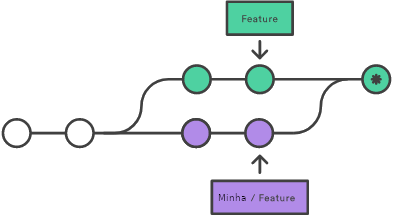
\includegraphics[width=0.7\textwidth]{imgGit/merge.png}
      \end{figure}
   	  Realizar uma mesclagem: \\
	  \codigo{git merge [branch]} \\[2mm]
  	  \textbf{Rebase}
  	  \begin{figure}[H]
        \centering
        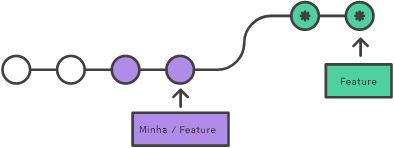
\includegraphics[width=0.7\textwidth]{imgGit/rebase.png}
      \end{figure}
	  Realizar um rebase: \\
      \codigo{git rebase [branch]} \\[2mm]
	  Parar uma rebase: \\
      \codigo{git abort [branch]} \\[2mm]
	  Resolver conflitos pela ferramenta: \\
      \codigo{git mergetool}
	\end{minipage}
  };  
  \node[fancytitle, right=10pt] at (box.north west) {Integrar Alterações da Ramificação};
\end{tikzpicture}

Página do GitHub: \url{https://github.com/}

\end{multicols*}
\end{document}